\documentclass[12pt]{article}
\usepackage[T1]{fontenc}
\usepackage[a4paper, total={7in, 10in}]{geometry}
\usepackage{graphicx}
\usepackage[export]{adjustbox}
\usepackage[font=normalsize,labelfont=bf]{caption}
\usepackage{caption}
\usepackage{subcaption}
\usepackage{float}
\usepackage{titling}
\usepackage{fancyhdr}
\usepackage{lipsum}

\title{Modernizacja Laboratorium Drgań}
\author{Mateusz Klisiewicz}
\newcommand{\mytitle}{PRZESTRZEŃ (PŁASZCZYZNA) FAZOWA}
\newcommand{\mysubtitle}{Modernizacja Stanowiska}
\fancyfoot{}
\fancyhead[L]{\mytitle}
\fancyhead[R]{\mysubtitle}

\fancyfoot[C]{\thepage}

\date{\today}



\renewcommand\maketitlehooka{\null\mbox{}\vfill}
\renewcommand\maketitlehookd{\vfill\null}
\renewcommand{\figurename}{Rysunek}
\graphicspath{{../tex_resources/}}
\title{\mytitle \\
  \large \mysubtitle}


\begin{document}
\pagestyle{fancy}
\maketitle
\newpage
\section{Wstęp}
\section{Kształt Eksperymentu}
\begin{figure}[h]
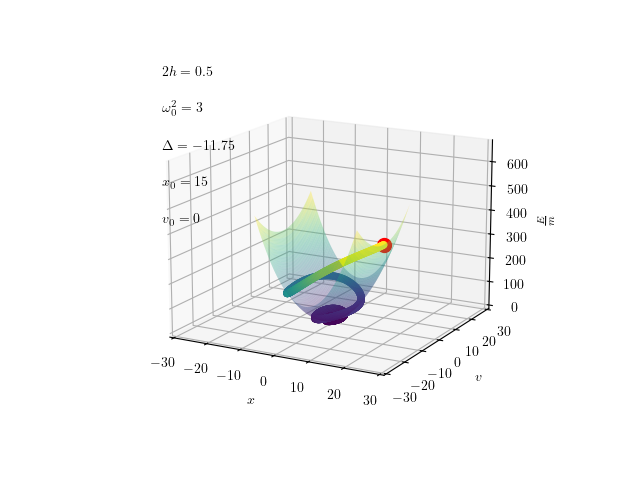
\includegraphics[width=16cm]{phase_plane_example}
\end{figure}
\begin{figure}[h]
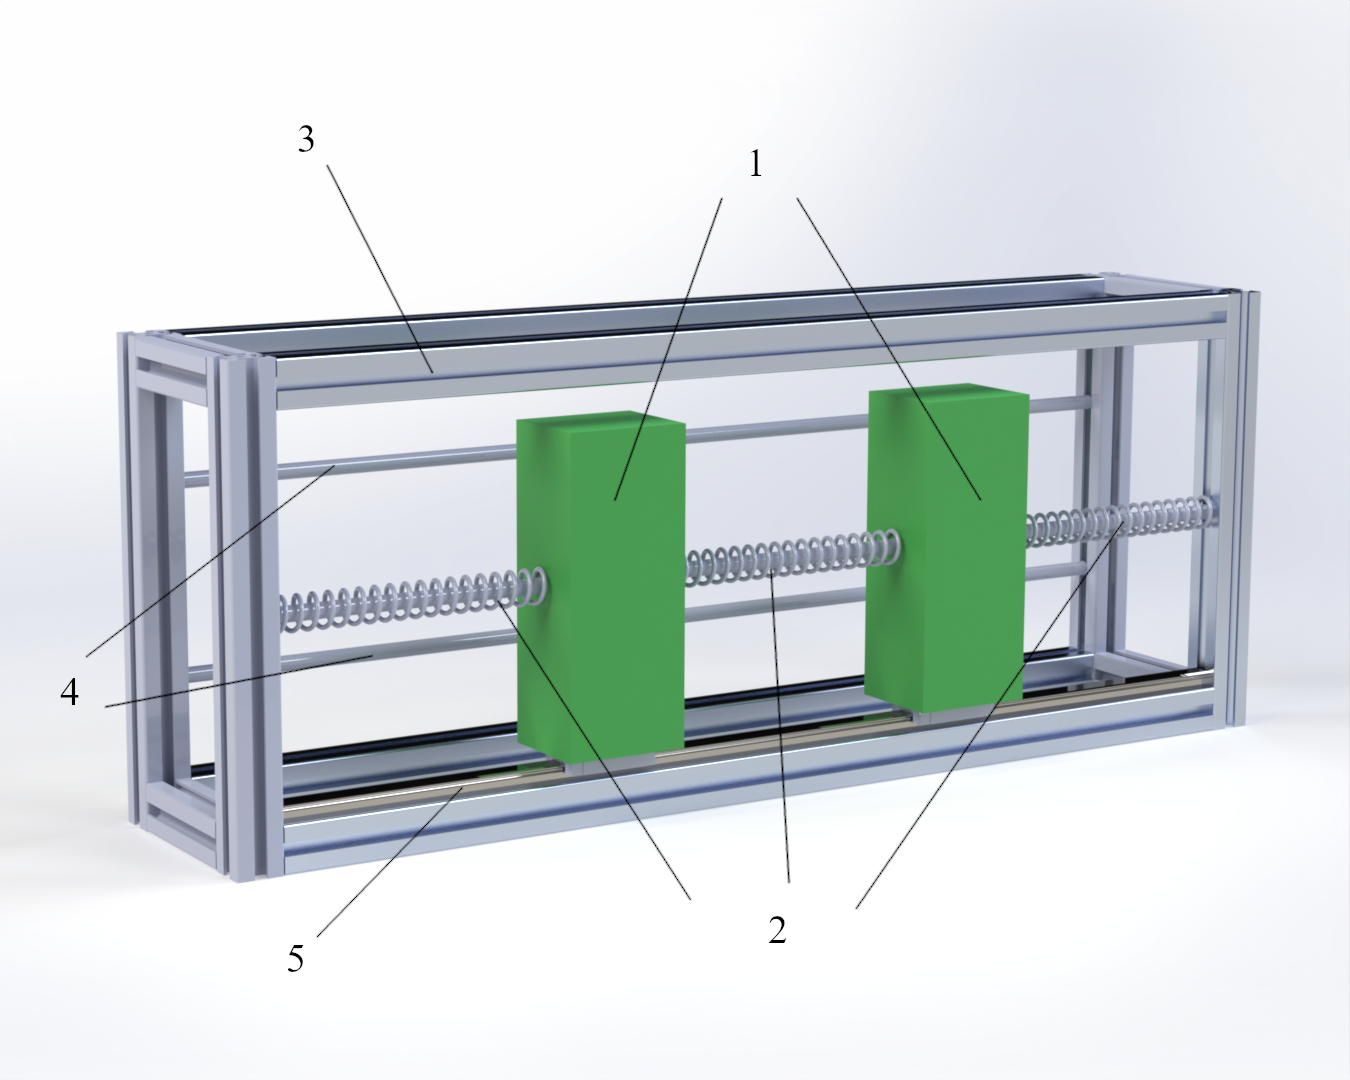
\includegraphics[width=16cm]{2dof_sch}
\end{figure}

\end{document}